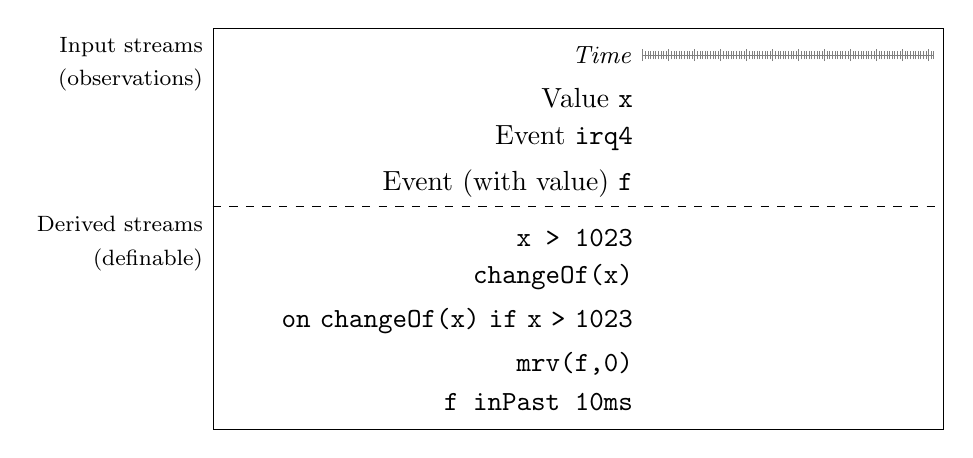
\begin{tikzpicture}

\matrix[column sep = 0.5em, draw] (m) {
  \node[anchor = east] {\small \textit{\textrm{Time}}}; \& \draw[help lines] (0,-0.05) grid[xstep=0.033] (3.7,0.05);
     \draw[gray] (0,-0.075) grid[xstep=0.33] (3.7,0.075); \\[0.5ex]
  \node[anchor = east] (m-1-2) {Value \texttt{x}}; \& \timing[name=m-2-2] at (0,-0.15) {2D{998}N(x1)2D{42}3D{2012}3D{1280}DD{10}DD{1404}};\\
%
  \node[anchor = east] (m-1-3) {Event \texttt{irq4}};
    \& \timing[name=m-2-3] at (0,-0.15) {ZZZ \n{} Z \n{} ZZZZ \n{} ZZ \n{} ZZZ \n{} Z}; \\
%
  \node[anchor = east] (end-inputs) {Event (with value) \texttt{f}};
    \& \timing[name = end-inputs-2] at (0,-0.15) {Z \n{17} ZZZZZZZ \n{98} Z \n{0} ZZZZ \n{23} Z}; \\[0.5em]
%
     \node[anchor = east] (m-1-5) {\texttt{x > 1023}};
  \& \timing[name=m-2-5] at (0,-0.15) {4L 6H 2L 2H}; \\
%
     \node[anchor = east] (m-1-6) {\texttt{changeOf(x)}};
  \& \timing[name=m-2-6] at (0,-0.15) {2Z \n{} 2Z \n{} 3Z \n{} 3Z \n{} 2Z \n{} 2Z}; \\
%
     \node[anchor = east, text width = 14.5em, align = right] (m-1-7) {
          \texttt{\textbf{on} changeOf(x) \textbf{if} x > 1023}};
  \& \timing[name=m-2-7] at (0,-0.15) {4Z \n{} 3Z \n{} 3Z 2Z \n{} 2Z}; \\
%
     \node[anchor = east] (m-1-8) {\texttt{mrv(f,0)}};
  \& \timing[name=m-2-8] at (0,-0.15) {D{0} 7D{17} D{98} 4D{0} D{23}}; \\
%
     \node[anchor = east] (m-1-9) {\texttt{f inPast 10ms}};
  \& \timing[name=m-2-9] at (0,-0.15) {L 2H 5L 3H 2L H}; \\
%
 };

\path[draw, dashed] (m.west|-end-inputs.south) edge (m.east|-end-inputs.south);

\path (m.north west) node[anchor = north east, align = right]
{\footnotesize{Input streams} \\ \footnotesize{(observations)}};

\path (m.west|-end-inputs.south) node[anchor = north east, align = right] {
  \footnotesize{Derived streams} \\ \footnotesize{(definable)}};

\end{tikzpicture}
